\documentclass{article}
\usepackage{url}
\usepackage{graphicx}
\usepackage{float}
\usepackage{biblatex}
\addbibresource{ref.bib}
\graphicspath{{./images}}
\title{Malware Reverse Engineering \\
Practical 2 Report \\
Spring 2022}
\author{Michael Ivanov \\
ivanovmichael@ufl.edu}
\date{March 14, 2022}

\begin{document}
    \maketitle
    \pagebreak
    \section{Executive Summary}
    \pagebreak
    \section{Static Analysis}

    \subsection{MD5 Hashes}
    \begin{itemize}
        \item sample2.exe: E05D85ACC62B2795BFB94A681E64E20F
        \item resource1 IDR{\_}X86BOT: 958596F72BD381520A75FFA6E4DB9827
        \item resource2 IDR{\_}X86LOADER: 27DA8F25FF1CB54C63618D2A489EE4DF
        \item resource3 IDR{\_}X86BOT: E8AF535C7447D203FF7CD44440B00459
        \item decoded IDR{\_}X86BOT: 1F1EDE22004510FB903D4CB45A769B12
    \end{itemize}

    \subsection{Program Compilation Date}
    \begin{itemize}
        \item sample2.exe: Fri Aug 19 09:54:32 2016
    \end{itemize}

    \subsection{Suspicious Imports}
    sample2.exe:
    \begin{itemize}
        \item \textbf{CreateProcessW:} This gives an indication the malware could be creating other processes.
        \item \textbf{TerminateProcess:}
        \item \textbf{VirtualProtect:} This can be used to change the permissions and protections of a process.
        \item \textbf{NtQueryInformationProcess:} Can be used to retrieve information about a specified process.
    \end{itemize}
    decoded.bin

    \subsection{Suspicious Strings}
    \begin{itemize}
        \item \textbf{"Wow64DisableWow64FsRedirection":} A function that disables file system redirection for the calling thread \cite{Wow64}.
        \item \textbf{"FindResource", "LoadResource":} Functions for finding and loading an external resource.
        \item \textbf{"Sleep":} Might be useful to know for later dynamic analysis, the program might hang for a long period of time.
        \item \textbf{".log"} A possible file extension to some kind of log file.
    \end{itemize}

    \subsection{Program sections}
    In the .rsrc (resource) section there are 3 files. I have provided the hashes above.

    \subsection{Anti-disassembly}
    \subsection{Program obfuscation}
    \begin{figure}[H]
        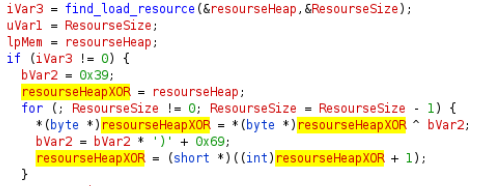
\includegraphics[width=\textwidth]{encodeXOR.png}
        \caption{Ghidra disassembly of potential resource obfuscation with XOR}
    \end{figure}

    \section{Dynamic Analysis}

    \subsection{Interesting behaviors}
    When the program is first executed it immediately deletes itself. However, by using Procmon I was able to see the program was still running. It was now in the \path{C:/Users/malware/AppData/Roaming} directory.
    \begin{figure}[H]
        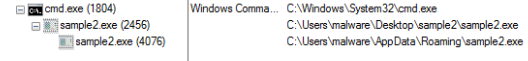
\includegraphics[width=\textwidth]{sample2process.png}
        \caption{Procmon showing the process tree of sample2.exe}
    \end{figure}

    \subsection{Contacted machines and services}
    \begin{itemize}
        \item HTTP GET \url{http://myexternalip.com/raw}
    \end{itemize}
    The above URL obtains the machine's external IP address. This may determine program behavior based on said IP address.
    \begin{figure}[H]
        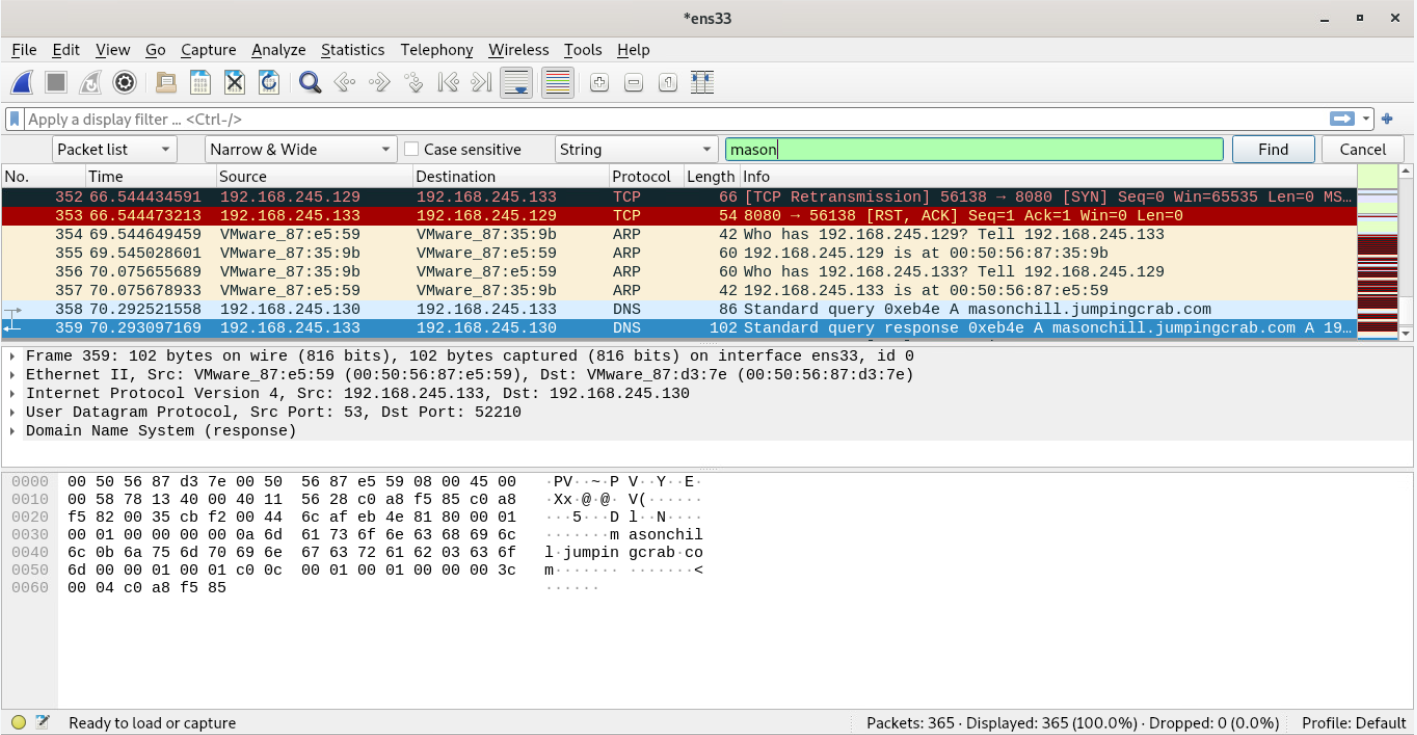
\includegraphics[width=\textwidth]{wireshark.png}
        \caption{Wireshark showing the HTTP get request from the above URL }
    \end{figure}
    \begin{figure}[H]
        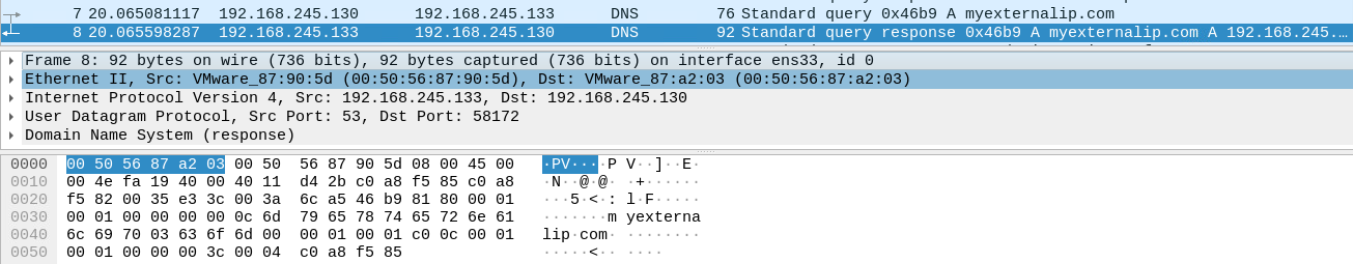
\includegraphics[width=\textwidth]{dns.png}
        \label{dns}
        \caption{Wireshark showing the DNS query and response }
    \end{figure}

    \subsection{Registry Keys created/modified}
    No registry keys were created or modified. However, the following key would have been created if it did not exist already.
    \begin{itemize}
        \item \path{HKLM\System\CurrentControlSet\Services\Tcpip\Parameters}
    \end{itemize}
    \begin{figure}[H]
        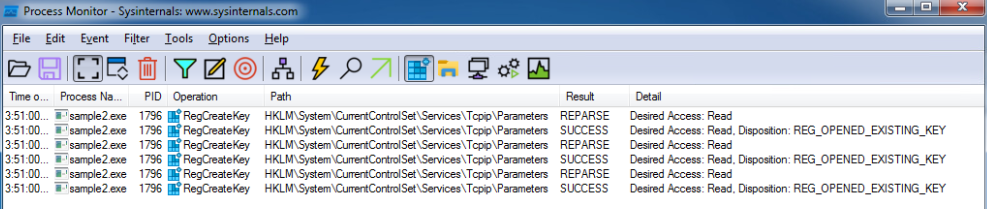
\includegraphics[width=\textwidth]{RegKeyCreate.png}
        \caption{Procmon showing the attempted creation of a registry key}
    \end{figure}

    \subsection{Files created/modified}
    Files Created:


    All instances of sample2.exe share the same hash.
    \begin{itemize}
        \item \path{C:\Users\malware\AppData\Roaming\sample2.exe}
        \item \path{C:\Users\System32\config\systemprofile\AppData\Roaming\sample2.exe}
        \item \path{C:\Users\System32\config\systemprofile\AppData\Roaming\client_id}
        \item \path{C:\Users\System32\config\systemprofile\AppData\Roaming\group_tag}
        \item \path{C:\Users\System32\config\systemprofile\AppData\Roaming\Modules}
    \end{itemize}
    \begin{figure}[H]
        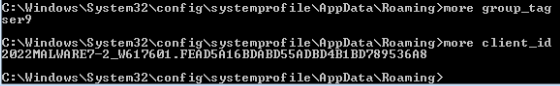
\includegraphics[width=\textwidth]{fileContents.png}
        \caption{The contents of the two new created files}
    \end{figure}
    \subsection{Processes started}
    \begin{itemize}
        \item \path{C:\Users\malware\AppData\Roaming\sample2.exe}
        \item \path{C:\Users\System32\config\systemprofile\AppData\Roaming\sample2.exe}
    \end{itemize}
    \begin{figure}[H]
        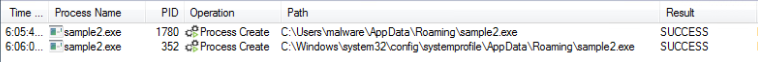
\includegraphics[width=\textwidth]{processCreated.png}
        \caption{Procmon showing the processes created by sample2.exe}
    \end{figure}

    \subsection{Persistence}
    \subsection{Deobfuscation}
    As seen in the static analysis obfuscation section, there was a suspicious for loop in the main function with a XOR operation. By examining the previous functions I was able to conclude that this loop was decoding a resource file by the name of IDR{\_}X86BOT. By stopping the debugger after this loop and dumping the data from address EDI till size ECX I was able to decode the binary. 
    \begin{figure}[H]
        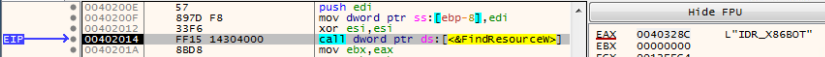
\includegraphics[width=\textwidth]{loadx86bot.png}
        \caption{Find and load of the encoded IDR{\_}X86BOT resource to be decoded later}
    \end{figure}
    \begin{figure}[H]
        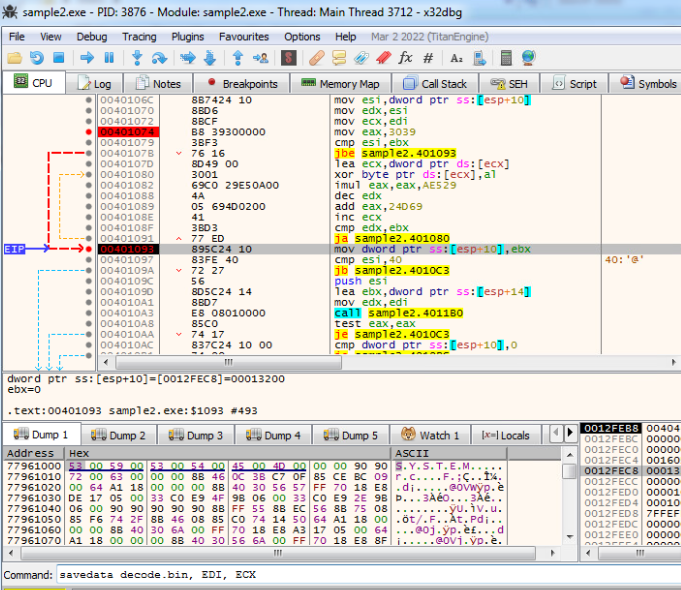
\includegraphics[width=\textwidth]{decode.png}
        \caption{Saving the decoded resource data from x32dbg with the "savedata" command}
    \end{figure}
    
    This new executable does not set or create any registry keys, but it does write to the same places as sample2.exe. Except it does not write to the "systemprofile" directory. However, this program has more networking traffic and contains different imports.
    \pagebreak
    \printbibliography

\end{document}